% !TeX root = ../main.tex

% DOCX body[3]
\section{Introduction}\label{sec:introduction}



% DOCX body[4]
Audio-visual generalized zero-shot learning (AVGZSL) jointly exploits the visual and audio streams of a video and establishes associations between audio-visual representations and textual class semantics. The goal is to recognize unseen classes that are absent from training while retaining the ability to distinguish seen classes. Representative methods, including CJME \cite{parida2020cjme}, AVGZSLNet \cite{mazumder2021avgzslnet}, AVCA \cite{mercea2022avca}, and ClipClap-GZSL \cite{kurzendorfer2024clipclap}, have attracted considerable attention in multimodal video understanding and demonstrated promising potential for unseen-class classification.

% DOCX body[5]
Most existing methods follow an \textquotedblleft{}encode first, match later\textquotedblright{} paradigm. They first extract visual and audio features using pre-trained models, encode these features into class-agnostic global representations with temporal Transformers (Fig.~\ref{fig:comparison}(a)) \cite{mercea2022tcaf} or cross-attention mechanisms (Fig.~\ref{fig:comparison}(b)) \cite{mercea2022avca}, and finally align the resulting representations with class label embeddings in a joint embedding space. However, this paradigm has three limitations. First, class semantics participate only in the final matching stage. Critical actions and sounds often occupy only a small portion of a long video, whereas class-irrelevant backgrounds, silence, and redundant movements dilute the discriminative evidence during uniform pooling. Second, although class label embeddings encode semantic relationships, they are not optimized for the target classification task. Closely situated class embeddings of similar classes consequently produce ambiguous decision boundaries. Third, audio and visual features are often concatenated directly or combined using a fixed fusion scheme. When the modalities are weakly correlated or one is noisy, irrelevant information can interfere across modalities and induce modality bias toward seen classes.



% DOCX body[12]
% DOCX body[12]
\begin{figure*}[pos=t]
\centering
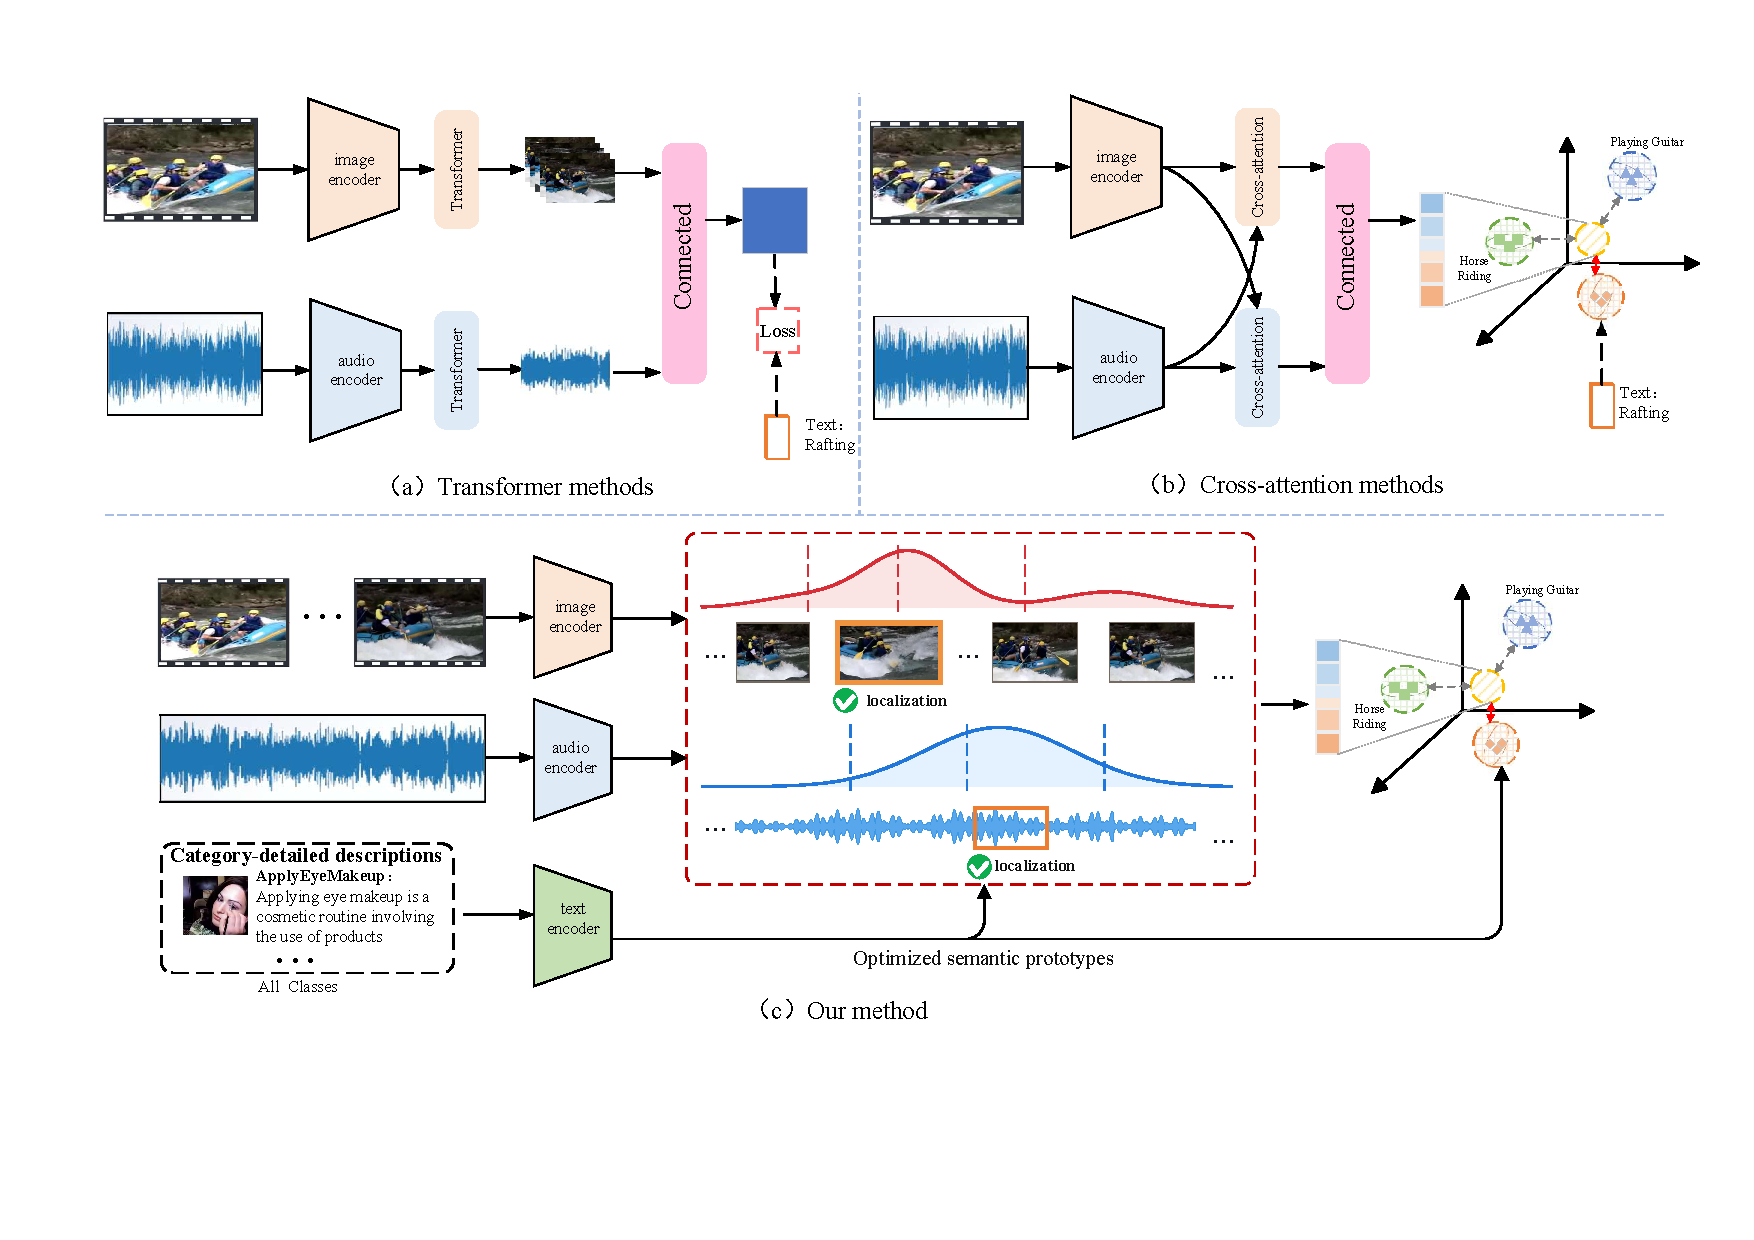
\includegraphics[pagebox=mediabox,width=\textwidth,trim={43bp 99bp 20bp 29bp},clip]{figures/Introduction.pdf}
\caption{Comparison of the proposed framework with existing AVGZSL methods. Transformer-based methods (a) emphasize intra-modal temporal modeling, whereas cross-attention-based methods (b) emphasize inter-modal interaction. Both follow the \textquotedblleft{}encode first, match later\textquotedblright{} paradigm without direct class-semantic guidance for temporal evidence selection. In contrast, our method (c) uses optimized class embeddings to guide independent Gaussian temporal aggregation for visual and audio sequences, adaptively localizes and aggregates class-relevant segments, and aligns the fused audio-visual representation with the class embeddings.}
\label{fig:comparison}
\end{figure*}


% DOCX body[6]
In this paper, we reconsider the role of class semantics in the recognition pipeline. Rather than treating semantics as static class embeddings used only for matching, we use them as active conditioning signals throughout temporal encoding, audio-visual grounding, and modality fusion. To this end, we propose SGTG, a framework for Semantic-Guided Gaussian Temporal Grounding for Audio-Visual Generalized Zero-Shot Learning. At its core, Class-Conditioned Gaussian Temporal Aggregation (CGTA) uses class-semantic queries to generate separate Gaussian distributions with predicted offsets from initial centers for the visual and audio sequences. Together with sample-adaptive routing weights, these distributions continuously localize, weight, and aggregate class-relevant segments. To provide reliable and transferable queries, we introduce Discriminative Semantic Prototype Optimization (DSPO), which improves class separability while preserving semantic structure. We further design Decoupled Modality Interaction and Gated Fusion (DMIF) to organize the aggregated evidence through separate intra-modal and inter-modal relationships. By adjusting fusion weights according to the sample and candidate class, DMIF makes effective use of the selected evidence.

% DOCX body[7]
These designs yield an AVGZSL framework centered on temporal grounding. Our main contributions are summarized as follows:

\begin{enumerate}
\renewcommand{\labelenumi}{(\arabic{enumi})}

% DOCX body[8]
\item We propose class-conditioned Gaussian temporal aggregation, which generates continuous Gaussian distributions conditioned on transferable class semantics and independently localizes and aggregates class-relevant segments along the visual and audio timelines.

% DOCX body[9]
\item We develop DSPO to optimize class embeddings under two competing objectives: class separability and semantic preservation. The learned class embeddings serve as both discriminative classification references and reliable queries for class-conditioned temporal aggregation.

% DOCX body[10]
\item We design decoupled modality interaction and gated fusion. Complementary attention masks separate intra-modal from inter-modal relationships, while candidate-class conditioning enables three-way adaptive weighting of intra-modal representations, inter-modal representations, and direct temporal evidence. This design mitigates interference caused by weak audio-visual correspondence and modality noise.

% DOCX body[11]
\item Experiments on three AVGZSL benchmarks, namely VGGSound-GZSL\textsuperscript{\textit{cls}}, UCF-GZSL\textsuperscript{\textit{cls}}, and ActivityNet-GZSL\textsuperscript{\textit{cls}}, demonstrate that the proposed model achieves state-of-the-art performance compared with existing methods.

\end{enumerate}
